\chapter{\ifcpe ทฤษฎีที่เกี่ยวข้อง\else Background Knowledge and Theory\fi}
\label{bg}

\section{Model View Controller (MVC)}
โครงงานนี้ใช้ design pattern MVC~\cite{mvc} ซึ่งแบ่งออกเป็น 3 ส่วนหลักๆ ดังรูปที่ \ref{mvc} ได้แก่ 
\begin{enumerate}
    \item Model
    \item View
    \item Controller
\end{enumerate}

  \begin{figure}[h!]
    \begin{center}
    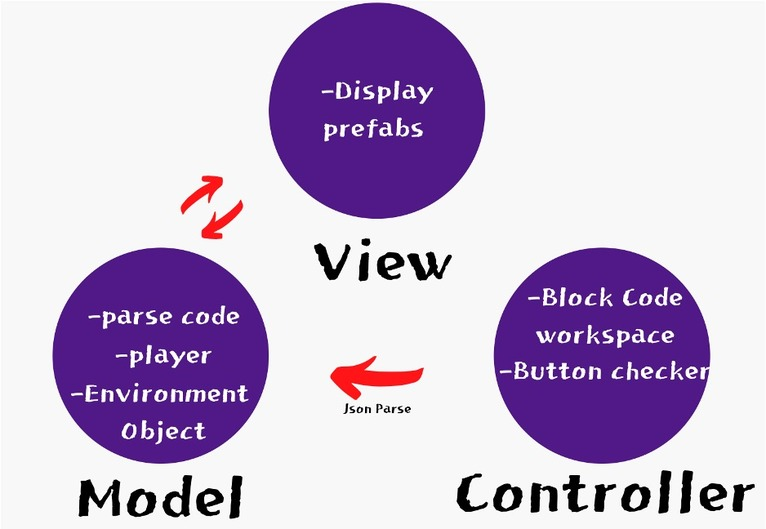
\includegraphics{pic/pic1.jpg}
    \end{center}
    \caption[Design Pattern MVC]{Design Pattern MVC}
    \label{mvc}
    \end{figure}
  

\subsection{Model}
 ในส่วนของ model จะเป็นการจัดการแปลงจาก block code ให้เป็น C\# เพื่อทำให้เกิด events ต่างๆ เช่นการเดิน การหมุน
 และการกระโดด เป็นต้น โดยที่ model จะรับ block code มาจาก controller ในรูปของ JSON
 และจะทำการแปลงเป็น C\# เพื่อสั่งให้ view แสดงผลต่างๆ ส่วนของ model จะอยู่ใน Unity
 เป็นตัวกลางในการสื่อสารระหว่าง view กับ controller

 \subsection{View}
 View นั้นทำหน้าที่เพียงแสดงผลโดยรับโค้ดคำสั่งมาจาก model แล้วทำการแสดงผล จากนั้นจะทำการ
 ส่งค่าคืน เพื่อแจ้ง model ว่าแสดงผลตามตามคำสั่งนั้นแล้ว ส่วนของ view จะอยู่ใน
 Unity เช่นกัน เพราะ view ใช้แสดงผลกราฟิกของ Unity ที่ผู้พัฒนาได้สร้างเอาไว้ เช่น prefabs(รูปแบบสำเร็จ) 
 ซึ่งเป็นวัตถุต่างๆ ภายในเกมที่ถูกสร้างขึ้นจาก Unity ให้มีคุณสมบัติตามที่ผู้พัฒนากำหนด ยกตัวอย่างเช่น ตัวละคร ก้อนหิน ดังรูปที่~\ref{prefabs}
 รวมไปถึงการแสดงหน้า UI ของเกม ซึ่งจะกล่าวถึงในหัวข้อ user interface
    

\subsection{Controller}
Controller จะอยู่ทั้ง 2 ฝั่ง คือทั้ง Unity และ WebView โดย controller ฝั่งหน้าเว็[ป]จะเป็นการรอให้ผู้ใช้
ลากวางตัว block code และเมื่อผู้ใช้กดรัน controller ฝั่งหน้าเว็บจะทำการแปลง block code ให้เป็น object 
ในรูปของ JSON และจะถูกนำส่งไปให้ controller ฝั่ง Unity หลักจากนั้น controller ฝั่ง Unity จะทำการ
ประมวลผลและแปลงเป็น object ที่ Unity สามารถอ่านได้เพื่อส่งต่อไปให้ model


\section{ระบบเกม}
เนื่องจากตัวเกมเสริมทักษะวิชาวิทยาการคำนวณที่ได้พัฒนานั้นมีระบบเกมที่ค่อนค่างแตกต่างจากระบบเกมด้วยทั่วๆ ไปเพราะว่าในตัวระบบเกมจะแบ่งการทำงานเป็นหลักๆ อยู่สองส่วนนั่นคือ WebView และ Unity
ซึ่งการทำงานของทั้งส่วนต้องมีการประสานงานกันถึงจะเกิดเป็นระบบเกมที่พัฒนาต้องการได้ ลุ่มโครงงานของพวกเราจึงได้ได้ใช้ภาษา C\#~\cite{cs} และ JavaScript~\cite{js}
ในการเขียนระบบเกมขึ้นมา โดยแบ่งเป็น 2 ส่วน ส่วนแรกคือ C\# ใน Unity 
และ ส่วนที่สองคือ JavaScript ใน WebView(ซึ่งจะกล่าวในหมวดเครื่องมือที่ใช้ในการทำ Blockly ใน Unity) โดยใช้ localhost ในการ host
\subsection{C\#}
C\# คือ ภาษาคอมพิวเตอร์ประเภท object-oriented programming พัฒนาโดย Microsoft โดยมีจุดมุ่งหมายในการวมความสามารถการคำนวณของ 
C++ ด้วยการโปรแกรมง่ายกว่าของ Visual Basic โดย C\# มีพื้นฐานจาก 
C++ และเก็บส่วนการทำงานคล้ายกับ Java 
C\# ได้รับการออกแบบให้ทำงานกับ .NET platform ของ Microsoft
จุดมุ่งหมายคือ อำนวยความสะดวกในการแลกเปลี่ยนสารสนเทศและบริการผ่านเว็บ 
และทำให้ผู้พัฒนาสร้างโปรแกรมประยุกต์ในขนาดกะทัดรัด C\# 
ทำให้โปรแกรมง่ายขึ้นผ่านการใช้ eXtensible Markup Language (XML) 
และ Simple Object Access Protocol (SOAP) 
ซึ่งยอมให้เข้าถึง objects ของโปรแกรมหรือ methods 
โดยปราศจากความต้องการให้ผู้เขียนโปรแกรมเขียนคำสั่งเพิ่มในแต่ละขั้นตอน 
เนื่องจากผู้เขียนโปรแกรมสามารถสร้างบนคำสั่งที่มีอยู่ 
แทนที่การคัดลอกซ้ำ C\# \newline
ภาษา C\#ถูกพัฒนาขึ้นโดยเป็นส่วนหนึ่งในการพัฒนาโครงสร้างพื้นฐานของ
.NET Framework เป็นการการนำข้อดีของภาษาต่างๆ 
(เช่น ภาษา Delphi, ภาษา C++) มาปรับปรุงเพื่อให้มีความเป็น OOP 
(โปรแกรมเชิงวัตถุ) มากขึ้น ขณะเดียวกันก็ลดความซับซ้อนในโครงสร้างของภาษาลง (เรียบง่ายกว่าภาษา C++) 
และมีสิ่งที่เกินความจำเป็นน้อยลง (เมื่อเทียบกับ Java)~\cite{cs}

โดยการที่เราศึกษาและเลือกใช้ ภาษา C\# เพราะว่ามีความเข้ากับตัวโปรแกรม 
Unity 3D ที่เราจะนำมาใช้ในการสร้างออกแบบ ตัวละคร และด่านต่างๆ ภายในเกม

\subsection{JavaScript}
JavaScript คือ ภาษาคอมพิวเตอร์สำหรับการเขียนโปรแกรมบนระบบอินเทอร์เน็ต 
เป็นภาษาสคริปต์เชิงวัตถุ ใช้ในการสร้างและพัฒนาเว็บไซต์ (ใช้ร่วมกับ HTML) 
ซึ่งมีวิธีการทำงานในลักษณะ object-oriented programming มีเป้าหมายในการ 
ออกแบบและพัฒนาโปรแกรมในระบบอินเทอร์เน็ต สำหรับผู้เขียนด้วยภาษา HTML 
สามารถทำงานข้ามแพลตฟอร์มได้ โดยทำงานร่วมกับภาษา HTML และภาษา Java 
ได้ทั้งทางฝั่งไคลเอนต์ (client) และ ทางฝั่งเซิร์ฟเวอร์ (server)

JavaScript ถูกพัฒนาขึ้นโดย เน็ตสเคปคอมมิวนิเคชันส์ 
(Netscape Communications Corporation) 
โดยใช้ชื่อว่า Live Script ออกมาพร้อมกับ Netscape Navigator~2.0 
เพื่อใช้สร้างเว็บเพจโดยติดต่อกับเซิร์ฟเวอร์
ต่อมาเน็ตสเคปจึงได้ร่วมมือกับ บริษัทซันไมโครซิสเต็มส์ปรับปรุงระบบ
ของบราวเซอร์เพื่อให้สามารถติดต่อใช้งานกับภาษา Java ได้~\cite{js}

ผู้พัฒนาได้ศึกษาและเลือกใช้ภาษา JavaScript เพราะ 
สามารถทำงานข้ามแพลตฟอร์มได้ โดยสามารถเข้าได้ทั้งกับ Unity และ WebView

\section{โปรแกรมที่ใช้ในการสร้างการออกแบบตัวเกม}
ตัวเกมในของโครงงานของพวกเรา ได้ใช้โปรแกรม Unity3d
ในการออกแบบ UX/UI ของตัวเกมขึ้นมาและทำกราฟฟิกในเกม 
ผ่านการใช้ assets ของ Unity และ การเขียน script 
โดยใช้ภาษา C\# ใช้ในการสร้างและพัฒนาเว็บไซต์

Unity คือ game engine ที่ช่วยสร้างเกม 3 มิติ 
และปัจจุบันก็สามารถเกม 2 มิติได้แล้วด้วย ซึ่ง 
สามารถทำงานได้ บน 2 แพลตฟอร์ม คือ Windows และ OSX 
และสามารถ export งานเพื่อนำไปใช้งานได้หลาย แพลตฟอร์ม 
เช่น Windows, OSX, Androids, iOS (iPhone) และ Web

Unity เป็นเครื่องมือช่วยสร้างเกมสามมิติและสองมิติ 
(ข้อแตกต่างระหว่างโลกสองมิติและสามมิติ คือแกน Z หรือความลึกที่เพิ่มเข้ามา 
พูดง่ายๆ ก็คือ นอกจากเราจะเคลื่อนที่ ขึ้น/ลง บนหน้าจอได้ ยังสามารถเคลื่อนที่ 
เข้าไปในจอได้)~\cite{unth}
\begin{itemize}
  \item Unity มองทุกอย่างเป็น game objects ไม่ว่าจะเป็นก้อนหินก้อนหนึ่ง 
  หรือ แมลงตัวหนึ่ง ถือเป็น game object โดย game object 
  จะทำงานร่วมกับ component game object ที่ปราศจาก component 
  ก็เหมือนฝุ่นผง ขยับ ไม่ได้ มองไม่เห็นด้วยตาเปล่า ซึ่ง component 
  เข้ามาเพิ่มคุณสมบัติและพฤติกรรมให้กับ game objects ให้สามารถเคลื่อนที่ได้ 
  เปล่งเสียงได้ เป็นต้น
  \item Game objects คือวัตถุต่างๆที่อยู่ในเกม 
  เช่น รถ 1 คัน, สัตว์ 1 ตัว, คน 1 คน, บ้าน 1 หลัง หรือ ต้นไม้ 1 ต้น เป็นต้น
  เช่น รถ 1 คัน, สัตว์ 1 ตัว, คน 1 คน, บ้าน 1 หลัง หรือ ต้นไม้ 1 ต้น เป็นต้น
  \item Components คือคุณลักษณะหรือความสามารถต่างๆ ของ objects เช่น การเคลื่อนไหว
  \item Assets คือ คุณลักษณะภายนอกที่เสริมการทำงานของ components
  \item Scene คือ ฉากแต่ละฉากซึ่งประกอบด้วย game objects หลายๆ ตัวรวมกัน
\end{itemize}

\section{เครื่องมือที่ใช้ในการทำ Blockly ใน Unity / เกมคอนโทรลเลอร์}
ตัวควบคุมเกมหลักของโครงงานของพวกเรา ได้ใช้ Blockly 
จาก Google for Education ในการทำส่วนของตัวเกมหลักที่ต้องมีการต่อชิ้นส่วน 
blocks โดยแต่ละ block ที่นำมาต่อกันนั้นพวกเราจะสร้างและพัฒนาขึ้นเอง ด้วยภาษา 
JavaScript ผ่าน WebView เพื่อนำไปใช้ในการแสดงผลบน Unity

\subsection{WebView}
เป็น asset ที่สามารถให้ผู้ใช้สามารถนำหน้าเว็บเข้าไปแสดงผลในตัวเกม Unity ได้~\cite{unw} โดย asset WebView จะจัดการฝังตัวหน้าเว็บที่ได้พัฒนาไว้และนำไปแสดงผลบน Unity UI panel

\subsection{Blockly}
Blockly เป็นผลิตภัณฑ์ของบริษัทกูเกิล ซึ่งมีโปรเจคของบริษัทหรือองค์กรไม่แสวงหากำไรต่างๆ นำไปพัฒนาต่อให้เข้ากับผลิตภัณฑ์ของตนเอง เช่น Scratch ที่ใช้ในการเรียนการสอนวิชาวิทยาการคำนวณ
และพวกเราเองก็นำมาใช้เช่นกัน Blockly 
เป็นเครื่องมือที่ช่วยให้การเขียนโปรแกรมนั้นง่ายขึ้นเพียงแค่ทำการลากแล้ววางเท่านั้น
Blockly เป็น library ที่สามารถเพิ่มตัวแก้ไขลงลงในแอปพลิเคชันของผู้ใช้ผ่านหลักการคิดการเขียนโปรแกรม
โดยแสดงผลโค้ดที่ถูกต้องตามหลักไวยากรณ์ในภาษาที่ผู้ใช้เลือก 
ช่วยให้ผู้ใช้สามารถใช้หลักการเขียนโปรแกรมโดยไม่ต้องกังวลเกี่ยวกับไวยากรณ์ 
สามารถใช้งานได้บนในเว็บไซต์ผ่านเครื่องคอมพิวเตอรหรือแอปพลิเคชันบนระบบปฏิบัติการ Android หรือ ระบบปฏิบัติการ iOS~\cite{blc}


\section{ความรู้ตามหลักสูตรซึ่งถูกนำมาใช้หรือบูรณาการในโครงงาน}
\begin{itemize}
  \item รู้จัก block code จากการเรียนรู้ในวิชา Basic Computer Engineering รหัสวิชา 261103 ซึ่งได้นำ block code มาใช้และเป็นแรงบันดาลใจในการทำโครงงานนี้ขึ้นมา
  \item ภาษา HTML และ JavaScript ได้รู้จักและเข้าใจพอสมควร จากการเรียนรู้ในวิชา Basic Computer Engineering Lab รหัสวิชา 261207 นำมาใช้กับการเขียนตัว controller ที่ใช้ควบคุม block code ผ่านการ hosting ด้วย localhost
  \item นำหลักการจากวิชา Object-Oriented Programming รหัสวิชา 261200 มาใช้ในการพัฒนาตัวเกมผ่าน Unity
\end{itemize}

\section{ความรู้นอกหลักสูตรซึ่งถูกนำมาใช้หรือบูรณาการในโครงงาน}
\begin{itemize}
  \item Unity พวกเราเห็นว่าน่าสนใจและเหมาะสมในการทำเกมเพราะสามารถสร้างเกมที่เป็น 3D จึงได้มีการศึกษาและค้นคว้าข้อมูลเพิ่มเติม รวมถึงฟังก์ชันและการใช้งานโดยรวมทั้งหมด
  \item การเปิด localhost บน Unity ผ่าน asset WebView
\end{itemize}

\begin{figure}[h!]
\begin{center}
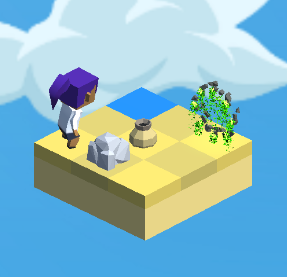
\includegraphics{pic/prefabs.png}
\end{center}
\caption[ตัวอย่าง prefabs ที่ใช้]{ตัวอย่าง prefabs ที่ใช้ }
\label{prefabs}
\end{figure}
